\documentclass{article}
\usepackage{graphicx} % Required for inserting images
\usepackage{amsfonts}
\usepackage{amsmath}
\usepackage{float}
\title{CSC311 Project Report}
\author{Ewan Jordan}
\date{April 2024}
\usepackage[legalpaper, margin=1in]{geometry}
\begin{document}

\maketitle

\section{Part A}
\subsection{}
\subsubsection{(a)}
\subsubsection{(b)}
\subsubsection{(c)}
\subsubsection{(d)}
\subsubsection{(e)}
\subsection{}
\subsubsection{(a)}
\subsubsection{(b)}
\subsubsection{(c)}
\subsubsection{(d)}
\subsection{(ii)}
\subsubsection{(a)}
Ok!
\subsubsection{(b)}
Final tuned hyperparameter values:\\
$k = 10$\\
$lr = 0.1$\\
$num\_epoch = 13$
\subsubsection{(c)}
Training objective as a function of epoch:\\
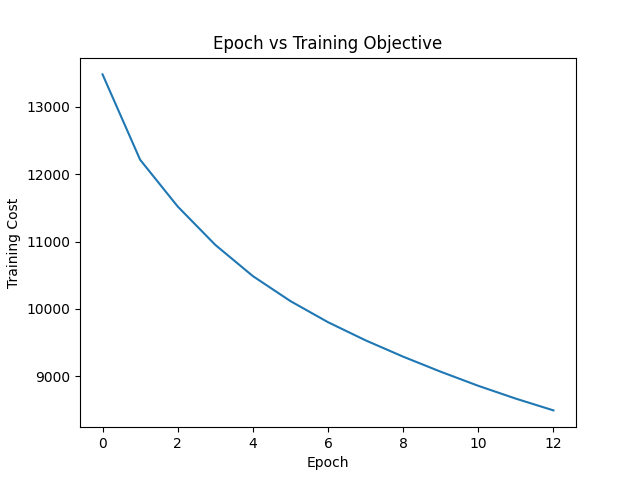
\includegraphics[scale=0.6]{figures/Aq3_train_objective_plot.png}\\
Validation objective as a function of epoch:\\
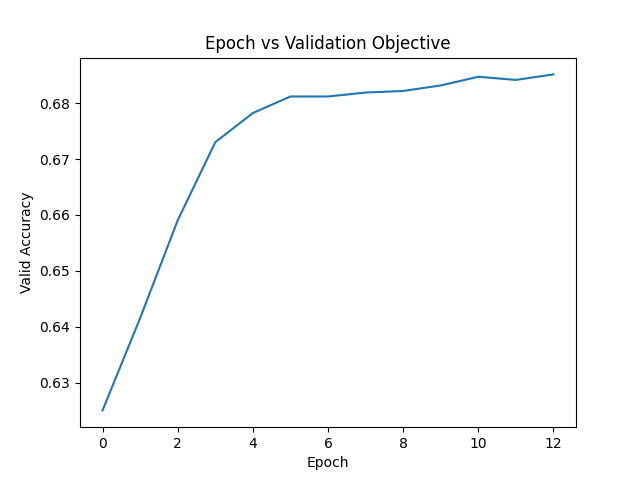
\includegraphics[scale=0.6]{figures/Aq3_valid_objective_plot.png}\\
\\
Test Accuracy: 0.6802145074795372
\subsubsection{(d)}
Final tuned lambda value:\\
$lamb = 0.001$\\
\\
Validation accuracy for final model: 0.6841659610499576\\
Test accuracy for final model: 0.6852949477843635\\
\\
Using a regularization penalty with our chosen $\lambda$, our model performs slightly better as the test accuracy increases by approximately 0.005.
\section{Part B}
\subsection{Formal Description of Algorithm}
Our team chose to modify the autoencoder used in Part A, question 3. We made several additions to the original, all which either centered around optimization improvements or attempts at reducing overfitting. We shall describe each modification in depth separately, and then the complete model visually.
\subsubsection{Training based on Questions}
The original model used as input the 584 student entities, each a tensor of length 1774 (each feature representing the students correctness on a question). For our modified model, we decided to reverse this and have our autoencoder take in the 1774 questions as input, each being a tensor of length 584 (each feature representing the correctness of a student's answer on this question). With this modification, the model's definition became,
Given a question $q \in \mathbb{R}^{N}$, $f$ is a reconstruction of the input $q$, where 

$$f(q, \theta) = h(W^{(2)}g(W^{(1)}q + b^{(1)}) + b^{(2)}) \in \mathbb{R}^{N_{\text{input}}}$$

Here, $W^{(2)} \in \mathbb{R}^{N_{\text{users}}\times k}$ and $W^{(1)} \in \mathbb{R}^{k\times N_{\text{users}}}$. $g$ and $h$ are still sigmoid functions. 

This change was motivated by the fact that we now have a higher number of data points, each with a lower number of features. We believe this could lead to a more accurate autoencoder, as there are less patterns to learn and more training data, which could theoretically strengthen the abilities of the network. We still tested out the rest of our modifications on both users and questions as entities. Proceeding, we use $N_{\text{input}}$ to abstractly represent $N_{\text{users}}$ and $N_{\text{questions}}$
\subsubsection{Additional Layers}
We have added additional layers in both the encoding and decoding process of the collaborative filtering. We have given these extra hidden layers a size of $2k$ after doing some testing, where $k$ is the size of our latent dimension. Let $\sigma$ denote the sigmoid function. This modification gives a new forward pass equation of,
$$L(x) = \sigma(H^{(1)}(\sigma(W^{(1)}x + b^{(1)}) + a^{(1)}) \in \mathbb{R}^{k}$$
$$f(x; \theta) = \sigma(W^{(2)}\sigma(H^{(2)}L(x) + a^{(2)}) + b^{(2)}) \in \mathbb{R}^N$$

Where $x$ is our input, either $\in \mathbb{R}^{N_{\text{users}}}$ or $\in \mathbb{R}^{N_{\text{questions}}}$, $N = |x|$, and $k$ is the size of the latent dimension. $W^{(2)} \in \mathbb{R}^{N_{\text{input}}\times 2k}$, $W^{(1)} \in \mathbb{R}^{2k\times N_{\text{input}}}$, $H^{(2)} \in \mathbb{R}^{2k\times k}$ and $H^{(2)} \in \mathbb{R}^{k\times 2k}$.

Deepening the network takes the same motivation as switching to question as entity; trying to improve the optimization. Adding layers in a neural network can improve performance because deeper neural networks can learn more complex, non-linear functions.
\subsubsection{Dropout}

Dropout is a regularization technique in neural networks aimed at preventing overfitting during training. It works by randomly removing neurons with a certain probability in each training iteration, forcing the network to learn more robust features independently and reducing dependency among neurons. This process effectively creates multiple sub-networks during training, leading to an ensemble effect that improves generalization. During evaluation, dropout is typically turned off, but the weights of connections are scaled to maintain consistency. This scaling is necessary because on a certain percentage of weights will be involved in each iteration of training, and thus will end up being much larger to account for the overall lack of latent input.
\begin{figure}[H]
    \centering
    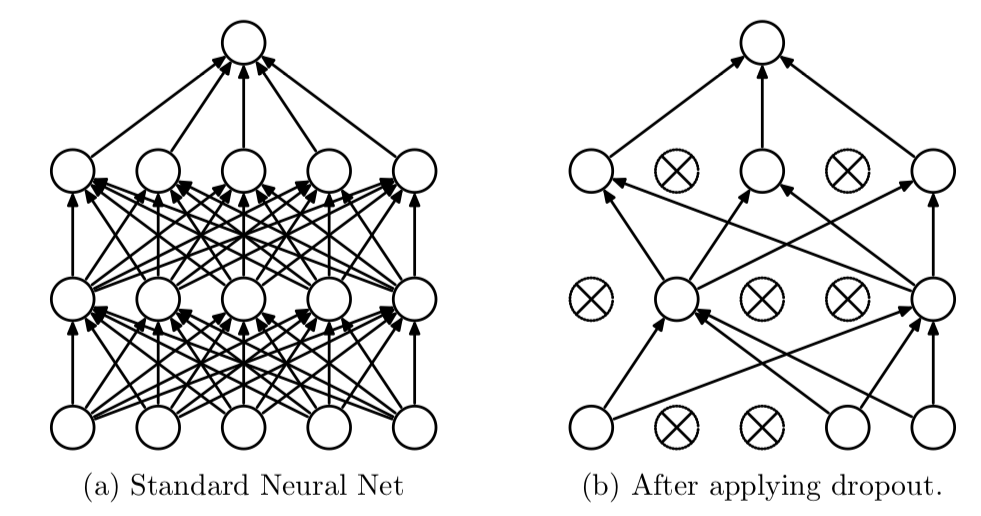
\includegraphics[width=0.5\linewidth]{dropout.png}
    \caption{Dropout — Srivastava et al. (2014)}
    \label{fig:enter-label}
\end{figure}

Figure 1 is what dropout looks like visually for a basic multilayer perceptron. We applied dropout to our autoencoder in each layer, in hopes to reduce overfitting and improve generalization.
\subsubsection{Dense Re-feeding}
One difficulty in training an autoencoder to perform collaborative filtering is the fact that training data is inherently sparse; Some data points will be missing values for certain features. However, we can take advantage of the fact that autoencoders output a vector of the same shape as the input, and use that output vector as a training data point of its own. As the model becomes more accurate these output vectors offer new opportunities for the model to consolidate its weights given vectors it has never seen before. 
\subsubsection{Meta-data Injection}
We took advantage of the meta data included in the data folder, in hopes at improving optimization. We believe there is useful relationships between the metadata and the behaviour of students on the questions, which hopefully can be picked up on by the network. We applied different techniques for inclusion of metadata in the case of training with students as entities and questions as entities.\\
We decided to have a stacked encoding layer of the network process meta data, then concatenate the latent representation of meta data with the latent representation of the original input vector x (again, either $x \in \mathbb{R}^{N_{\text{input}}}$ or $x \in \mathbb{R}^{N_{\text{questions}}}$). This latent concatenation was then fed into the decoder to produce our output vector. Additionally, in the case of question meta data, we preprocess the data to be a onehot encoding of the question's subject list; $X_{meta} \in \mathbb{I}^{N_{\text{questions}}\times N_{subjects}}$. The mathematical representation for question as entity is as follows,
$$E_{meta}: \mathbb{I}^{N_{\text{subjects}}} \rightarrow \mathbb{R}^{k_{meta}}$$
$$E_{meta}(x_{meta}) = T^{(1)}x_{meta} + t^{(1)}$$
$T^{(1)} \in \mathbb{R}^{k_{\text{meta}} \times N_{\text{subjects}}}$
$$E_{\text{question}}(q): \text{Latent representation of question}$$
$$f(q) = \text{Decode}(\text{Concatenate}(E_{meta}(x_{meta}), E_{\text{question}}(q)))$$
Where Decode is the decoder network, as defined within the Additional Layers section.
\subsubsection{IRT Beta Injection}
When performing IRT collaborative filtering, we learn latent beta values for each question, relating to the supposed difficulty of each question. If this pretrained value is fed to the network for each question, it could theoretically be used to gain more information about the expected correctness of students' answers on the question. The value is fed into the network in the latent layer in the same way at the metadata, except now there is no additional network to encode the value.
\subsection{Model Diagram}
The final autoencoder we came up with incorporates all the modifications listed above.
\begin{figure}[H]
\centering
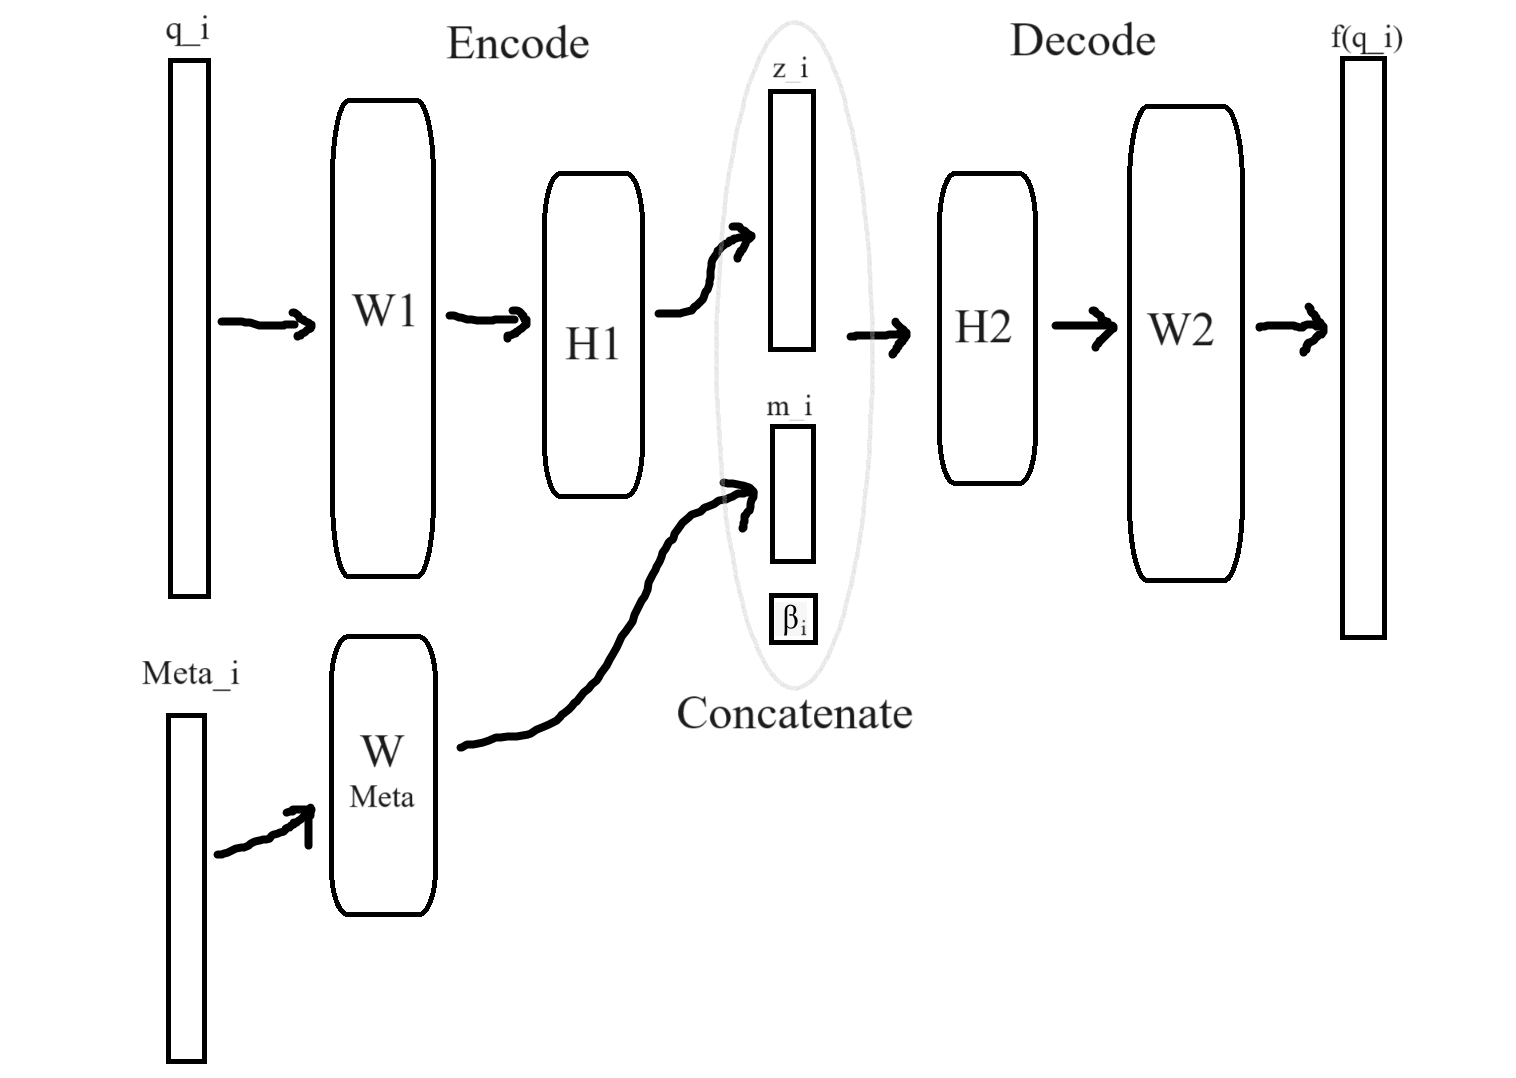
\includegraphics[width=1
\linewidth]{model.png}
\caption{Diagram of Model during Evaluation/Inference}
\label{fig:enter-label}
\end{figure}

\begin{figure}[H]
    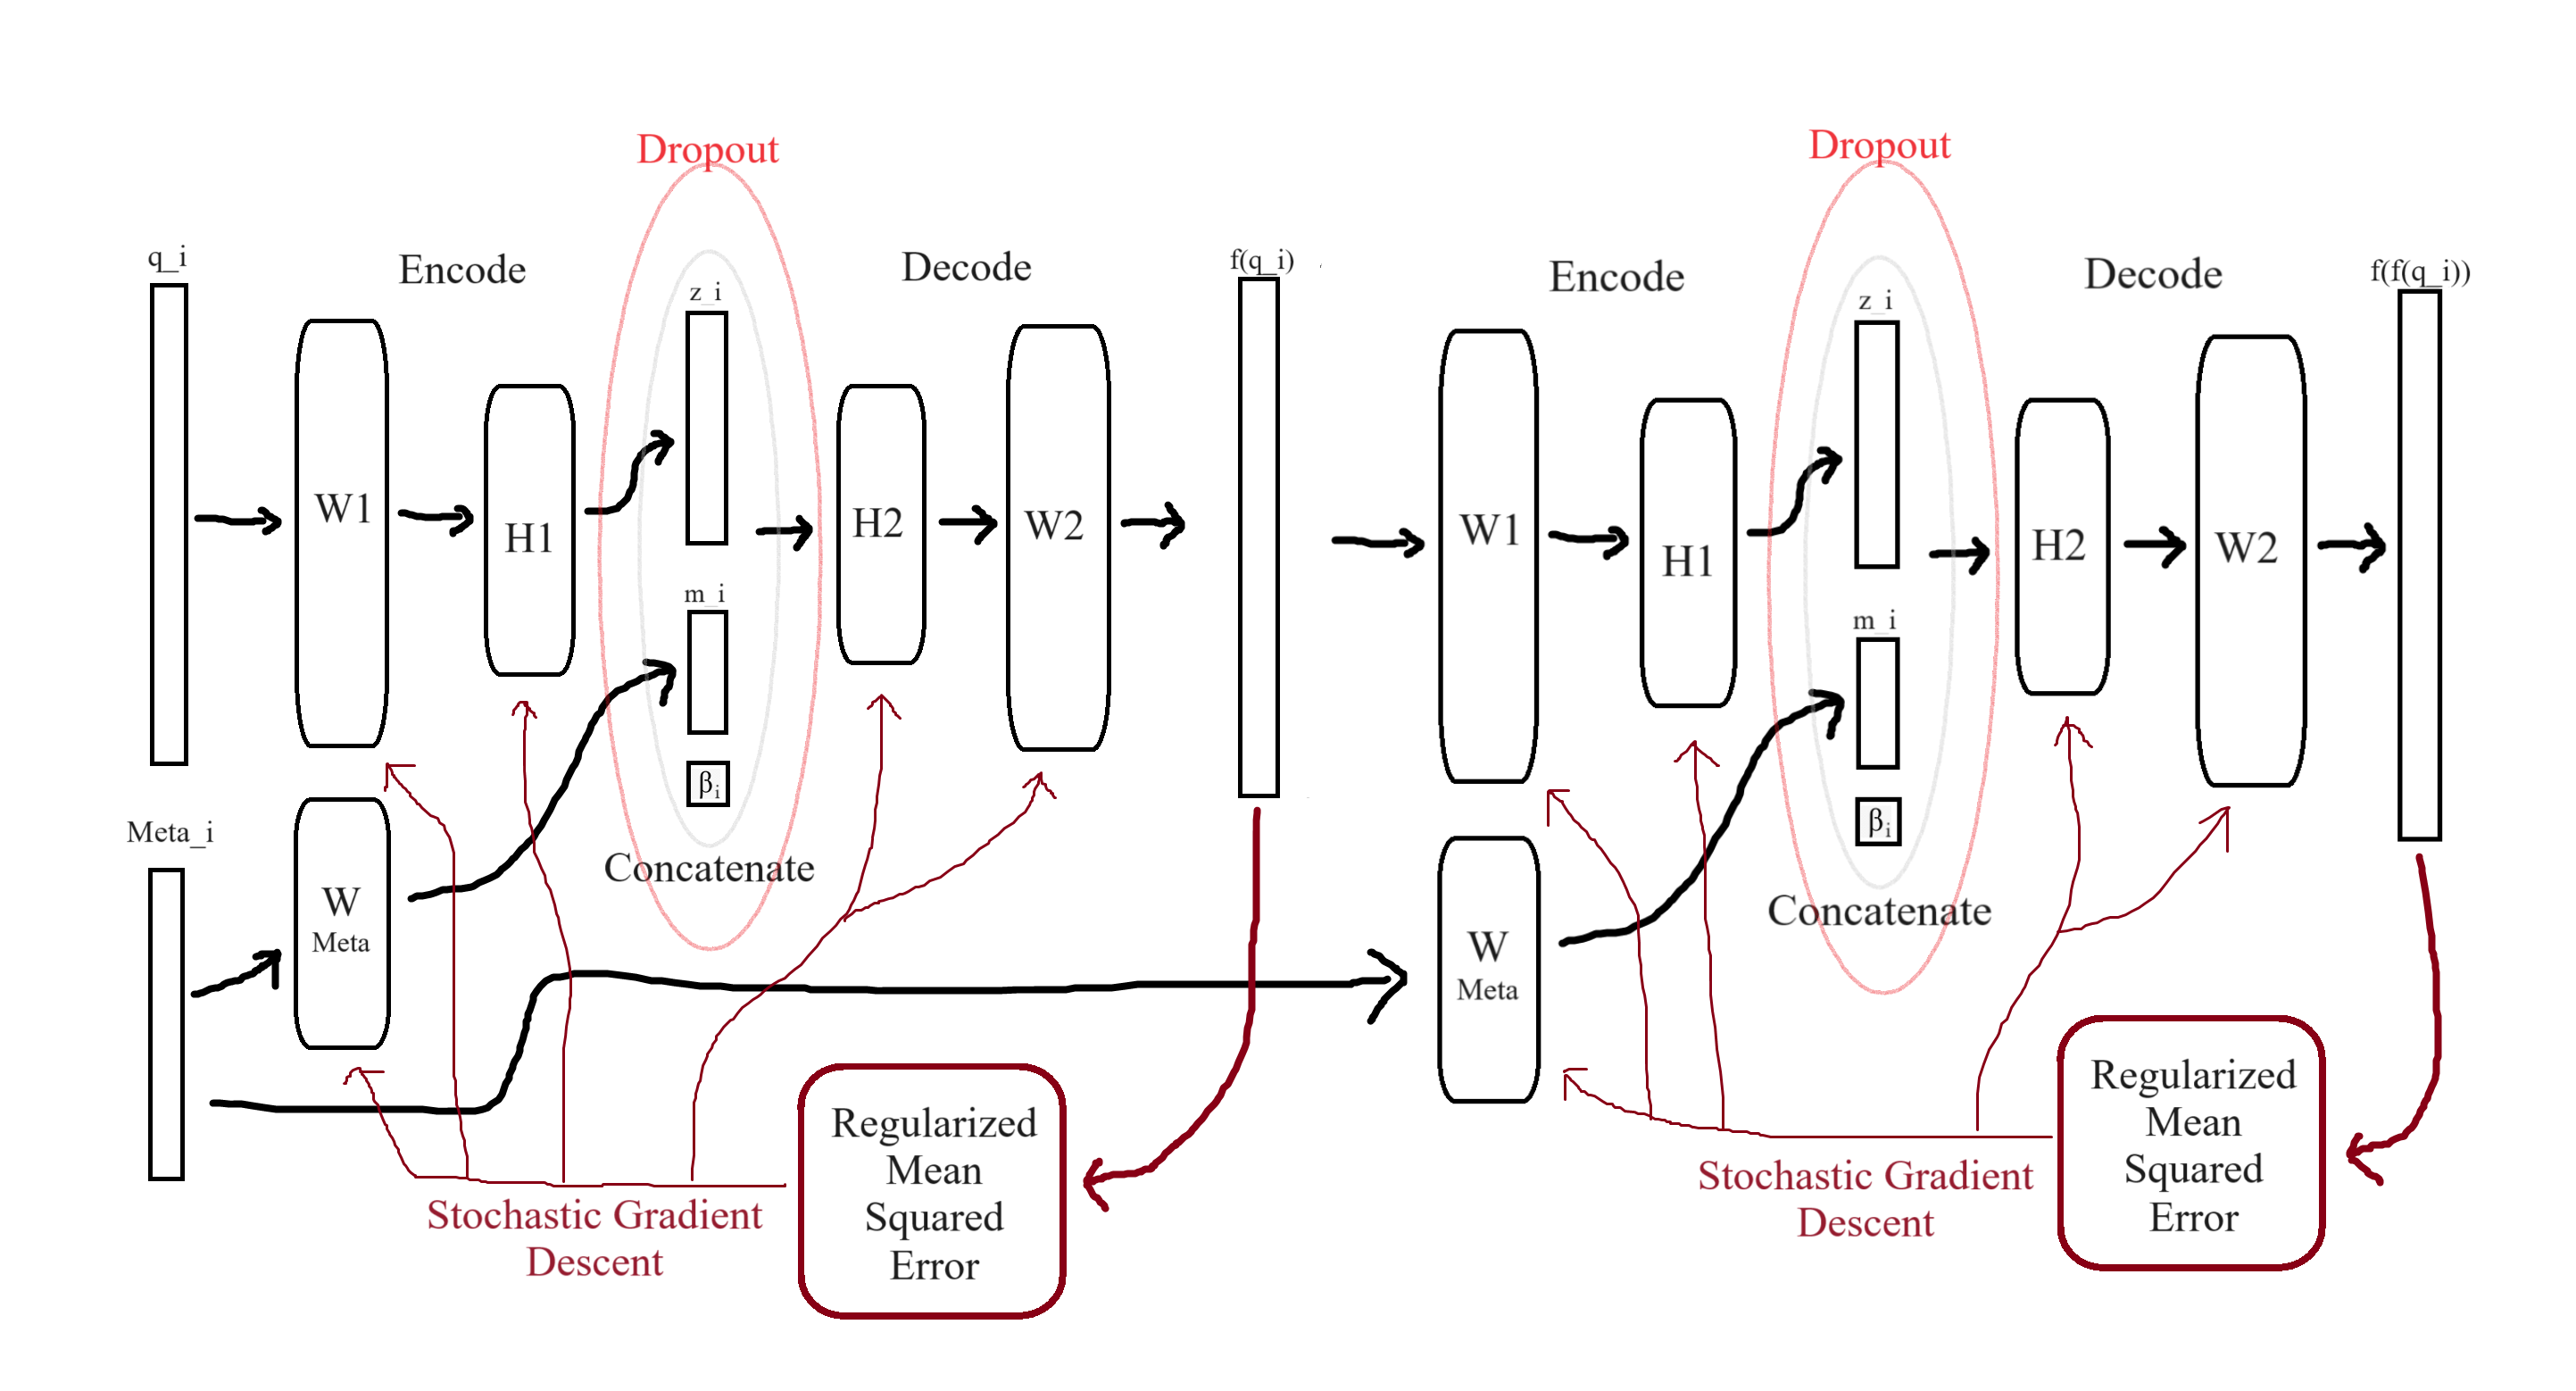
\includegraphics[width=\textwidth,height=\textheight,keepaspectratio]{model during training.png}
    \caption{Diagram of Model during Training}
    \label{fig:enter-label}
\end{figure}
\newpage

N. Srivastava, G. Hinton, A. Krizhevsky, I. Sutskever, R. Salakhutdinov, “Dropout: A Simple Way to Prevent Neural Networks from Overfitting” (2014)

\end{document}
